\documentclass[hyperref={pdfpagelabels=true}]{beamer}

\usepackage{verbatim}
\usepackage{graphicx}
\usepackage{amsfonts}
\usepackage{amstext}
\usepackage{amsmath}
\usepackage{amssymb}
\usepackage{mathrsfs}
\usepackage{rotating}
\usepackage{multicol}
\usepackage{color}
\usepackage{hyperref}
\usepackage{colortbl}
\usepackage{longtable,array}
\usepackage{booktabs}
%\usepackage{Sweave}

\definecolor{lb}{rgb}{0.5,0.8,0.98}
\definecolor{or}{rgb}{1,0.37,0.1}
\definecolor{llb}{rgb}{0.7,0.9,1}
\definecolor{lor}{rgb}{1,0.55,0.35}
\definecolor{llor}{rgb}{1,0.75,0.55}
\definecolor{lllor}{rgb}{1,0.85,0.65}
\definecolor{llllor}{rgb}{1,0.95,0.75}
\definecolor{lllllor}{rgb}{1,0.975,0.85}



\mode<presentation>{\usetheme{default}}
\usepackage[latin1]{inputenc}
\usepackage{times}
\usepackage[T1]{fontenc}

\title{Bayesian Model Averaging}
\subtitle{Journal Club}
\institute[Institut für Biostatistik]{Institute of Biostatistics\\ \url{andreaskitsche@gmail.com}}
\author{Andreas Kitsche}
\date{21. November 2011} 

\setbeamercovered{dynamic}


\begin{document}

%\setbeamertemplate{navigation symbols}{\footnotesize
%\setbeamertemplate{navigation symbols}{}

\setbeamertemplate{blocks}[rounded][shadow=true]
\addtocounter{framenumber}{-1}

\begin{frame}
\titlepage
\end{frame}






\begin{frame}
\frametitle{Multivariate data}
\begin{table}
	\centering
		\begin{tabular}{cccc} \hline
		Unit & Variable 1 & $\ldots$ & Variable p\\ \hline
		1 & $x_{11}$ & $\cdots$ & $x_{1p}$\\
		$\vdots$ & $\vdots$ & $\vdots$ & $\vdots$ \\
		n&$x_{n1}$ & $\ldots$ & $x_{np}$ \\ \hline
		\end{tabular}
\end{table}
Observed values are stored in the data matrix  \boldmath$X$ \unboldmath:

\begin{align*}
\bf X = \begin{pmatrix}
x_{11} &  \cdots & x_{1p}\\
\vdots & \vdots &\vdots  \\ 
x_{n1} & \cdots & x_{np}
\end{pmatrix}
\end{align*}

\nocite{Genell.2010}
%\nocite{Wasserman.2000}
\nocite{Raftery.1997}
\nocite{Hoeting.2000}
\nocite{Clyde.1999}
%\nocite{Daimon.2011}
\nocite{PENROSE.1985}

\end{frame}

\begin{frame}
\frametitle{Variable Selection and Linear Regression}
\begin{itemize}
\item given a dependent variable Y
\item given a set of candidate predictors $X_{1},\ldots,X_{k}$
\item find the best regression model of the form
\[
Y = \beta_{0} + \sum_{j=1}^{p}\beta_{i_{j}}X_{i_{j}} + \epsilon, \hspace{1cm} \epsilon \sim N(0, \sigma^{2}I)
\]
where $X_{i_{1}},\ldots,X_{i_{p}}$ is a subset of $X_{1},\ldots,X_{k}$\\
\item use the model to proceed effect sizes and standard errors
\item make predictions
\end{itemize}
\vspace{0.5cm}
"A typical approach to data analysis is to carry out a
model selection exercise leading to a single "best" model
and then to make inferences as if the selected model were
the true model (the selected model generated the data)." [Raftery et al. (1997)]
\end{frame}

\begin{frame}
\frametitle{Model Uncertainty and Bayesian Model Averaging}
\textcolor{red}{Problem}: uncertainty in model selection, leading to over-confident inferences
and decisions that are more risky than one thinks they are.\\
\vspace{0.5cm}
\textcolor{red}{"part of the evidence is spent to specify the model"}
\vspace{0.5cm}\\
BMA seeks to average over all possible sets of predictors
\end{frame}


\begin{frame}
\frametitle{Bayesian data analysis}
The Bayes´rule:
\[
\underbrace{p(\theta|D)}_{posterior}
=
\underbrace{p(D|\theta)}_{likelihood}
\underbrace{p(\theta)}_{prior}
/
\underbrace{p(D)}_{evidence} 
\]
where the evidence (maginal distribution, prior predictive) is
\[
p(D) = \int d\theta p(D|\theta)p(\theta)
\]
\begin{itemize}
\item prior $p(\theta)$ the strength of our belief in $\theta$ without the data
\item posterior $p(\theta|D)$ the strength of our belief in $\theta$ when the Data $D$ have been taken into account
\item likelihood $p(D|\theta)$ the probability that the data could be generated by the model with parameter values $\theta$
\item evidence $p(D)$ the probability of the data according to the model, determined by summing across all possible parameter values weighted by the strength of belief in those parameter
\end{itemize}
\end{frame}


\begin{frame}
\frametitle{Bayesian data analysis for model selection}
suppose we have two models $M1$ and $M2$, then Bayes´ rule is:
\[
p(M1|D) = p(D|M1)p(M1)/p(D) 
\]
\[
p(M2|D) = p(D|M2)p(M2)/p(D)
\]
The ratio of these is
\[
\frac{p(M1|D)}{p(M2|D)} = 
\underbrace{\frac{p(D|M1)}{p(D|M2)}}_{Bayes factor}
\frac{p(M1)}{p(M2)}
\]
\end{frame}


\begin{frame}
\frametitle{Bayesian model averaging}
\begin{itemize}
\item$M$ = $\left\{M_{1},\ldots,M_{K}\right\}$ - the set of all models being considered
\item $\Delta$- quantity of interest, i.e. effect size (the parameter estimate divided by its standard error)
\item $D$ - data
\end{itemize}
Posterior distribution of $\Delta$ is an average of the posterior distributions under each of the models considered, weighted by their posterior model probabilities:
\[
Pr(\Delta|D) = \sum_{k=1}^{K}Pr(\Delta|M_{k},D)Pr(M_{k}|D),
\]
where the posterior probability of model $M_{k}$ is given by
\[
Pr(M_{k}|D)=\frac{Pr(D|M_{k})Pr(M_{k})}{\sum_{l=1}^{k}Pr(D|M_{l})Pr(M_{l})}
%Pr(M_{k}|D)=\int Pr(D|\theta_{k},M_{k})Pr(\theta_{k}|M_{k})d\theta_{k}
\]
\end{frame}

\begin{frame}
\frametitle{Bayesian model averaging}
\[
Pr(D|M_{k})=\int Pr(D|\theta_{k},M_{k})Pr(\theta_{k}|M_{k})d\theta_{k}
\]
with:
\begin{itemize}
\item $Pr(D|M_{k})$ the marginal likelihood of model $M_{k}$
\item $\theta_{k}$ vector of parameters of model $M_{k}$
\item $Pr(\theta_{k}|M_{k})$ the prior density of $\theta_{k}$ under model $M_{k}$
\item $Pr(D|\theta_{k},M_{k})$ the likelihood
\item $Pr(M_{k})$ the prior pobability that $M_{k}$ is the true model
\end{itemize}
\end{frame}

\begin{frame}
\frametitle{Posterior model probability}
Suppose that $(K +1)$ models, $M_{0},M_{1},\ldots,M_{K}$are being considered.\\
Each of $M_{1},\ldots,M_{K}$ is compared in turn with $M_{0}$, yielding Bayes' Factors $B_{10},\ldots,B_{K0}$.\\
Then the posterior probability of $M_{k}$ is:
\[
pr(M_{k}|D)=\alpha_{k}B_{k0}/\sum_{r=0}^{K}\alpha_{r}B_{r0}
\]
where $\alpha_{k}=pr(M_{k})/pr(M_{0})$ is the prior odds for $M_{k}$ against $M_{0}$
\end{frame}

\begin{frame}
\frametitle{Specifying prior model probabilities}
A prior probability on model $M_{i}$ can be specified as:
\[
pr(M_{i})=\prod_{j=1}^{p}\pi_{j}^{\delta_{ij}}(1-\pi_{j})^{1-\delta_{ij}}
\]
where $\pi_{j} \in [0,1]$ is the prior probability that $\beta_{j}\neq 0$ in a regression model, and $\delta^{ij}$ is an indicator of whether or not variable $j$ is included in model $M_{i}$
\begin{itemize}
\item $\pi_{j}=0$ for all $j$ - uniformed prior across model space
\item $\pi_{j}<0.5$ for all $j$ - imposes a penalty for large models
\item $\pi_{j}=1$ - variable $j$ is included in all models
\end{itemize}
\end{frame}


\begin{frame}
\frametitle{Occam´s Window \cite{Madigan.1994}}
Building a subset of models\\
\begin{enumerate}
\item Exclude models not belonging to:
\[
A'= \left\{M_{k}: \frac{max_{l}\left\{Pr(M_{l}|D)\right\}}{Pr(M_{k}|D)}\leq C\right\},
\]
where $C$ is chosen by the data analyst and $max_{l}\left\{Pr(M_{l}|D)\right\}$ denotes the model with the highest posterior model probability
\item exclude models that receive less support from the data than any of their simpler submodels:
\[
B = \left\{M_{k}: \exists M_{l} \in M, M_{l}\subset M_{k}, \frac{Pr(M_{l}|D)}{Pr(M_{k}|D)} > 1 \right\}
\]
\end{enumerate}
\end{frame}

\begin{frame}
\frametitle{Occam`s Window}
%\[
%Pr(\Delta|D) = \frac{\sum_{M_{k}\in A} Pr(\Delta|M_{k},D) Pr(D|M_{k}) Pr(M_{k})}{\sum_{M_{k}\in A} Pr(D|M_{k}) Pr(M_{k})},
%\]
%where
%\[
%A = A'\backslash B \in M
%\]
%When the algorithm compares two nested models
%and decisively rejects the simpler model, then
%all submodels of the simpler model are rejected.\\
%Interpretation of the ratio of posterior model probabilities 
$M_{0}$ is smaller than $M_{1}$\\
If there is evidence for $M_{0}$ then $M_{1}$ is rejected, but
rejecting $M_{0}$ requires strong evidence for the larger
model, $M_{1}$.
\[
\frac{pr(M_{0}|D)}{pr(M_{1}|D}
\]
\begin{figure}
	\centering
		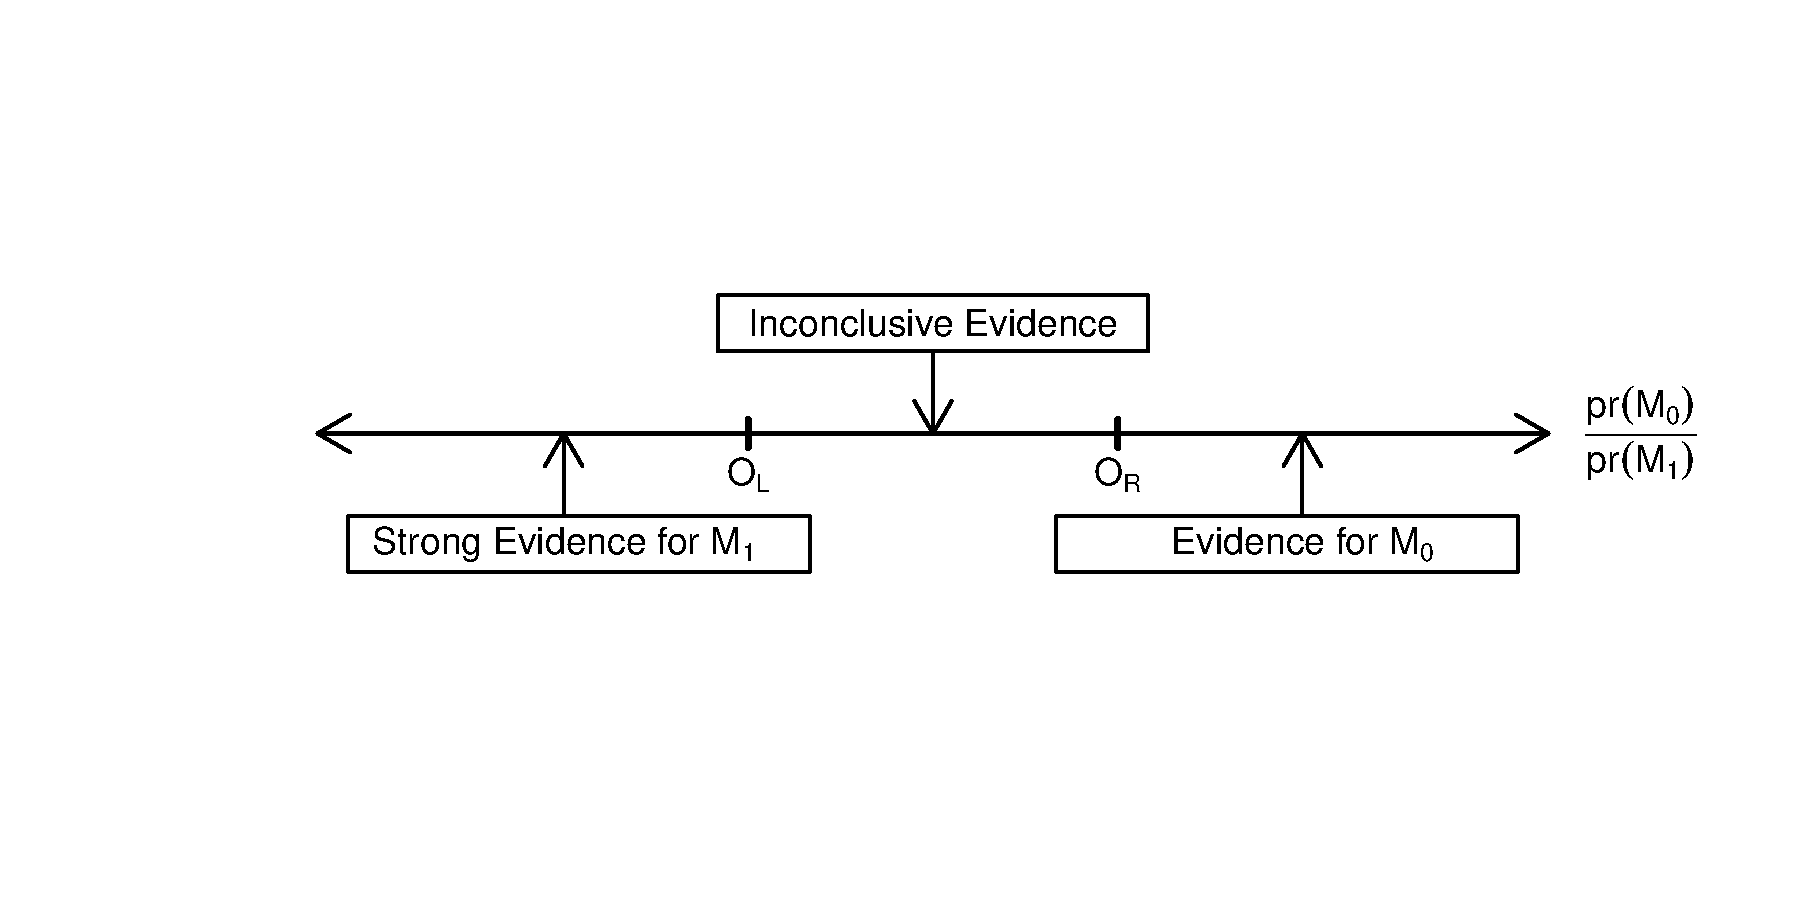
\includegraphics[width=1.00\textwidth]{OccamsWindow}
	\label{fig:OccamsWindow}
\end{figure}
choose $O_{L}$ and $O_{R}$ to 1/20 and 20
\end{frame}

\begin{frame}
\frametitle{Markov Chain Monte Carlo Model Composition ($MC^{3}$)}
Method developed by \cite{Madigan.1995}
\begin{itemize}
\item generate a stochastic process which moves through the model space 
\item Construct a Markov chain $\left\{M(t),t=1,2,\ldots,\right\}$ with state space $M$ and equilibrium distribution $pr(M_{i}|D)$
\item define the function $g(M_{i})$ on $M$ and simulate the Markov chain $t=1,\ldots,N$
\item $\hat{G}=\frac{1}{N}\sum_{t=1}^{N}g(M(t))$ is a simulation-consistent estimate of $E(g(M))$ as $N \rightarrow\infty$
\item define $g(M)=pr(\Delta|M,D)$
\end{itemize}
\end{frame}

\begin{frame}
\frametitle{Markov Chain Monte Carlo Model Composition ($MC^{3}$)}
\begin{itemize}
\item define the neighborhood $nbd(M)$ for each $M \in M$ that consists of the model M itself and the state of models with either one variable more or one variable fewer than $M$
\item define a transition matrix $q$ by setting $q(M \rightarrow M')=0$ for all $M' \notin nbd(M)$ and $q(M \rightarrow M')$ constant for all $M' \in nbd(M)$
\item in state $M$ we proceed by drawing $M'$ from $q(M) \rightarrow M')$
\item accept with probability 
\[
min\left\{1,\frac{Pr(M'|D)}{Pr(M|D)}\right\}
\]
\end{itemize}
\end{frame}

\begin{frame}
\frametitle{R implementation for BMA}
R package \texttt{BMA} \\
available functions 
\begin{itemize}
\item \texttt{bis.glm(x,...)} - Bayesian Model Averaging for generalized linear models
\item \texttt{bic.surv(x,...)} - Bayesian Model Averaging for Cox proportional hazards models for censored survival data
\item \texttt{bicreg(x,...)} - Bayesian Model Averaging for linear regression models
\item \texttt{plot(bicreg,...)} -  plot of the posterior distribuion of the coefficients produced by model averaging
\end{itemize}
Limitations: including an ad hoc model selection criterion that may bias posterior estimates
\end{frame}%\footnotesize

\begin{frame}
\frametitle{R implementation for BMA}
R package \texttt{BAS} \\
For p less than 20-25, BAS can enumerate all models depending on memory availability
Bayesian Model Averaging using Bayesian Adaptive Sampling
\begin{itemize}
\item \texttt{bas.lm(x,...)}
\begin{itemize}
\item \texttt{modelprior} - Family of prior distribution on the models
\item \texttt{initprobs} - vector of length p with the initial inclusion probabilities
\end{itemize}
\end{itemize}
Advantages: 
\begin{itemize} 
\item it can search very large model spaces
\item it offers a variety of prior specification options
\end{itemize}
Limitations: BAS can only estimate ordinary least squares
\end{frame}

\begin{frame}
\frametitle{Predicting Percent Body Fat [Penrose et al. (1985)]}
A data frame containing the estimates of the percentage of body fat determined by underwater
weighing and various body circumference measurements for 252 men.
\tiny
\begin{itemize}
\item case - case number
\item brozek - Percent body fat using Brozek's equation: 457/Density - 414.2
\item siri - Percent body fat using Siri's equation: 495/Density - 450
\item density - density determined from underwater weighing ($gm/cm^{3}$)
\item age - Age (years)
\item weight - Weight (lbs)
\item height - Height (inches)
\item neck - Neck circumference (cm)
\item chest - Chest circumference (cm)
\item abdomen - Abdomen circumference (cm)
\item hip - Hip circumference (cm)
\item thigh - Thigh circumference (cm)
\item knee - Knee circumference (cm)
\item ankle -Ankle circumference (cm)
\item biceps - Biceps (extended) circumference (cm)
\item forearm - Forearm circumference (cm)
\item wrist - Wrist circumference (cm) 
\end{itemize}
\end{frame}


\section{References}
\setcounter{page}{1}
\pagenumbering{roman}
\footnotesize
\bibliographystyle{plainnat}
\bibliography{JournalClub_BMA}
\end{document}



